% This file was created with tikzplotlib v0.9.17.
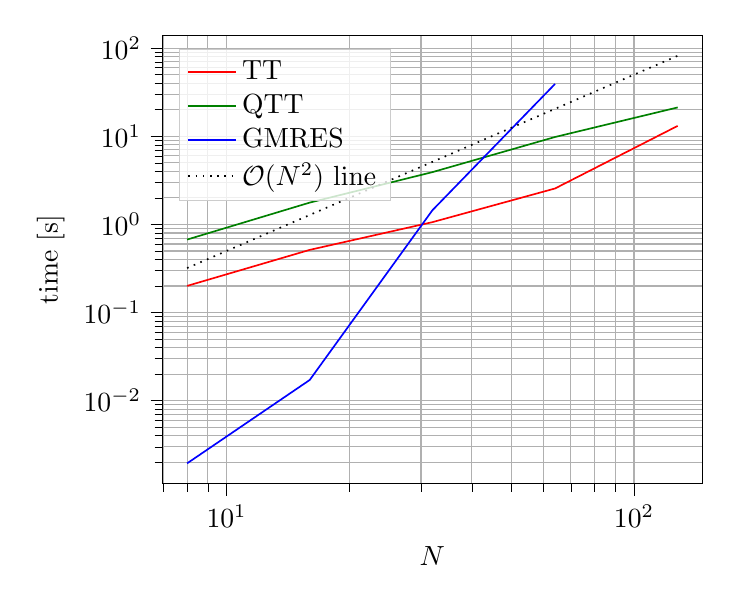
\begin{tikzpicture}

\begin{axis}[
legend cell align={left},
legend style={
  fill opacity=0.8,
  draw opacity=1,
  text opacity=1,
  at={(0.03,0.97)},
  anchor=north west,
  draw=white!80!black
},
log basis x={10},
log basis y={10},
tick align=outside,
tick pos=left,
unbounded coords=jump,
x grid style={white!69.0196078431373!black},
xlabel={\(\displaystyle N\)},
xmajorgrids,
xmin=6.96440450636899, xmax=147.03338943962,
xminorgrids,
xmode=log,
xtick style={color=black},
y grid style={white!69.0196078431373!black},
ylabel={time [s]},
ymajorgrids,
ymin=0.00114207884945846, ymax=139.512609024808,
yminorgrids,
ymode=log,
ytick style={color=black}
]
\addplot [semithick, red]
table {%
8 0.200653
16 0.514338
32 1.061089
64 2.55754
128 13.126228
};
\addlegendentry{TT}
\addplot [semithick, green!50!black]
table {%
8 0.673283
16 1.769102
32 3.920333
64 9.815639
128 21.257514
};
\addlegendentry{QTT}
\addplot [semithick, blue]
table {%
8 0.001945
16 0.017183
32 1.44627
64 39.240734
128 nan
};
\addlegendentry{GMRES}
\addplot [semithick, black, dotted]
table {%
8 0.32
16 1.28
32 5.12
64 20.48
128 81.92
};
\addlegendentry{$\mathcal{O}(N^{2})$ line}
\end{axis}

\end{tikzpicture}
